% !TeX spellcheck = en_US
\documentclass[a4paper,11pt]{scrartcl}

%\renewcommand{\arraystretch}{1.5}


%\lvsemester{SS 2021}
%\lvname{Computational Linguistics}
%\zeit{60 minutes}
%\datum{July 21\textsuperscript{th} 2021}

\usepackage{graphicx}
\graphicspath{
    {.} % document root dir
    {images/}
}

\usepackage{enumitem}
\usepackage[outputdir=out]{minted}
\usepackage[dvipsnames]{xcolor} % to access the named colour LightGray
\definecolor{LightGray}{gray}{0.9}


% Load the setspace package
\usepackage{setspace}
% Using \doublespacing in the preamble 
% changes text to double line spacing
\doublespacing


\title{W8 Assignment -- Machine Learning 3}
\subtitle{Computational Linguistics}

\author{John Gamboa}
\date{\today}

\setkomafont{author}{\sffamily}
\setkomafont{date}{\sffamily}



\setlength{\parindent}{0pt}


%% Adapted from
%% https://tex.stackexchange.com/questions/179197/framed-or-colored-box-with-text-and-margin-notes
%\usepackage[many]{tcolorbox}
%\newtcolorbox{story}[1][]{
%  top=-10pt,
%  width=\textwidth,
%  fonttitle=\bfseries,
%  breakable,
%  %boxrule=10pt,
%  %extrude right by=4cm,
%  fonttitle=\bfseries\color{Brown},
%  colframe=LightGray,
%  colback=LightGray!10,
%  #1}



\begin{document}
\maketitle

\section{Overfitting}

The following graph shows the development of the accuracy of a model as the
number of iterations of the Gradient Descent algorithm increases.

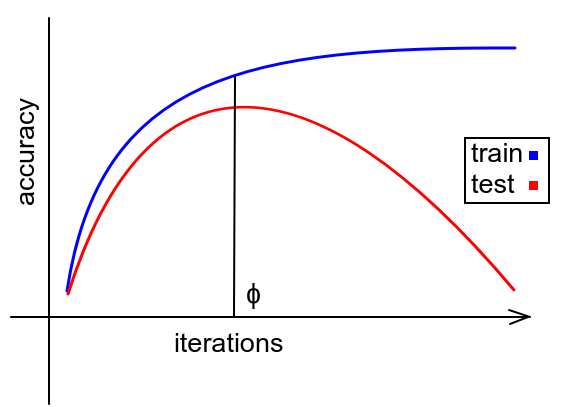
\includegraphics[width=0.6\textwidth]{overfitting}


The accuracy of the model on both the training and the test set are presented
for various numbers of iterations. The point $\Phi$ indicates the iteration
from which the red graph starts to increase again.

Based on this graph, it is possible to say that...
(choose \textit{TRUE} or \textit{FALSE})

\begin{enumerate}[label=\alph*)]
\singlespacing%\onehalfspacing

\item As the iterations increase, the model keeps fitting better and better
      the test set

\verb|answer|: \_\_\_\_\_\_\_\_\_\_\_\_\_\_\_\_\_\_\_\_\_\_\_\_\_\_\_\_\_\_\_\_

\item From around the iteration $\Phi$, the model starts to overfit 

\verb|answer|: \_\_\_\_\_\_\_\_\_\_\_\_\_\_\_\_\_\_\_\_\_\_\_\_\_\_\_\_\_\_\_\_

\item As the iterations increase, the model keeps fitting better and better
      the training set

\verb|answer|: \_\_\_\_\_\_\_\_\_\_\_\_\_\_\_\_\_\_\_\_\_\_\_\_\_\_\_\_\_\_\_\_

\item When training the model, we should repeatedly calculate the performance
      of the model both on the training and on the test set, so that we can
      find the point when the model starts overfitting

\verb|answer|: \_\_\_\_\_\_\_\_\_\_\_\_\_\_\_\_\_\_\_\_\_\_\_\_\_\_\_\_\_\_\_\_

\item The performance of the model on the test set always better than the
      performance of the model on the training set

\verb|answer|: \_\_\_\_\_\_\_\_\_\_\_\_\_\_\_\_\_\_\_\_\_\_\_\_\_\_\_\_\_\_\_\_

\item As the model overfits, it loses its ability to generalize to new
      (unseen) data

\verb|answer|: \_\_\_\_\_\_\_\_\_\_\_\_\_\_\_\_\_\_\_\_\_\_\_\_\_\_\_\_\_\_\_\_

\item The "best" model (i.e., the model that we would like to keep) is at or
      around the iteration $\Phi$

\verb|answer|: \_\_\_\_\_\_\_\_\_\_\_\_\_\_\_\_\_\_\_\_\_\_\_\_\_\_\_\_\_\_\_\_

\end{enumerate}


\section{Artificial Neuron}

\subsection{Threshold}

The image below shows the output of an artificial neuron for several different
inputs $X0$ and $X1$. The activation function of this neuron is such that it
will output $0$ if its input is below a certain threshold $\Phi$; and it will
output $1$ if its input equals or is above the threshold $\Phi$.

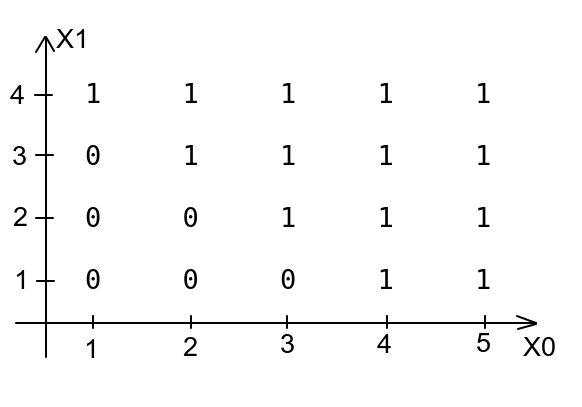
\includegraphics[width=0.6\textwidth]{neuron_output}

Consider that $W0 = 1$ and $W1 = 1$, and assume that the threshold is an integer
number. What is the threshold $\Phi$ of this neuron?

$~~\bigcirc$ 1
$~~\bigcirc$ 2
$~~\bigcirc$ 3
$~~\bigcirc$ 4
$~~\bigcirc$ 5
$~~\bigcirc$ None of the others



\subsection{Threshold + weights}

The image below shows the output of an artificial neuron for several different
inputs $X0$ and $X1$. The activation function of this neuron is such that it
will output 0 if its input is below a certain threshold $\Phi$; and it will
output 1 if its input equals or is above the threshold $\Phi$.

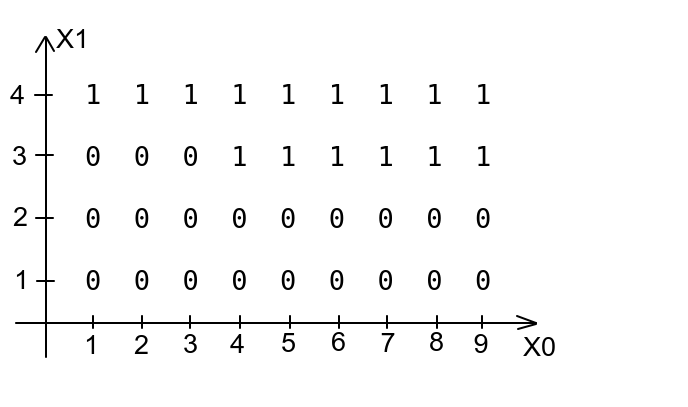
\includegraphics[width=0.6\textwidth]{neuron_output2}

Consider that $W0 = 0.2$ and $W1 = 1.5$, and assume that the threshold is an
integer number. What is the threshold $\Phi$ of this neuron?

$~~\bigcirc$ 1
$~~\bigcirc$ 2
$~~\bigcirc$ 3
$~~\bigcirc$ 4
$~~\bigcirc$ 5
$~~\bigcirc$ None of the others


\section{POS Tagging}

\subsection{Coding}

Consider the following piece of code:

{\singlespacing
\begin{minted}[bgcolor=LightGray,fontsize=\footnotesize]{python}
import nltk
sentence = "I like bacon with chocolate"

tagged = nltk.pos_tag(sentence)

[p[1] for p in tagged]
\end{minted}
}

What is this code doing?
(choose the correct alternative)

\begin{itemize}
\singlespacing
\item Outputting all the words of the sentence

\item Making a list with the POS tags, out of order, associated to each of the words in the sentence

\item Making a list containing all the pairs (word, POS tag) associated, in order, with each of the words in the sentence

\item Making a set with all the POS tags associated to each of the words in the sentence

\item Making a list with the POS tags, in order, associated to each of the words in the sentence

\item Getting only the second element of the sentence and putting it in a list
\end{itemize}

\verb|answer|: \_\_\_\_\_\_\_\_\_\_\_\_\_\_\_\_\_\_\_\_\_\_\_\_\_\_\_\_\_\_\_\_

\end{document}

